\chapter{Introduction}\label{chapter:introduction}

\epigraph{Weather forecast for tonight: dark.}{\textit{George Carlin}}

\begin{wrapfigure}{l}{0.4\textwidth}
    \centering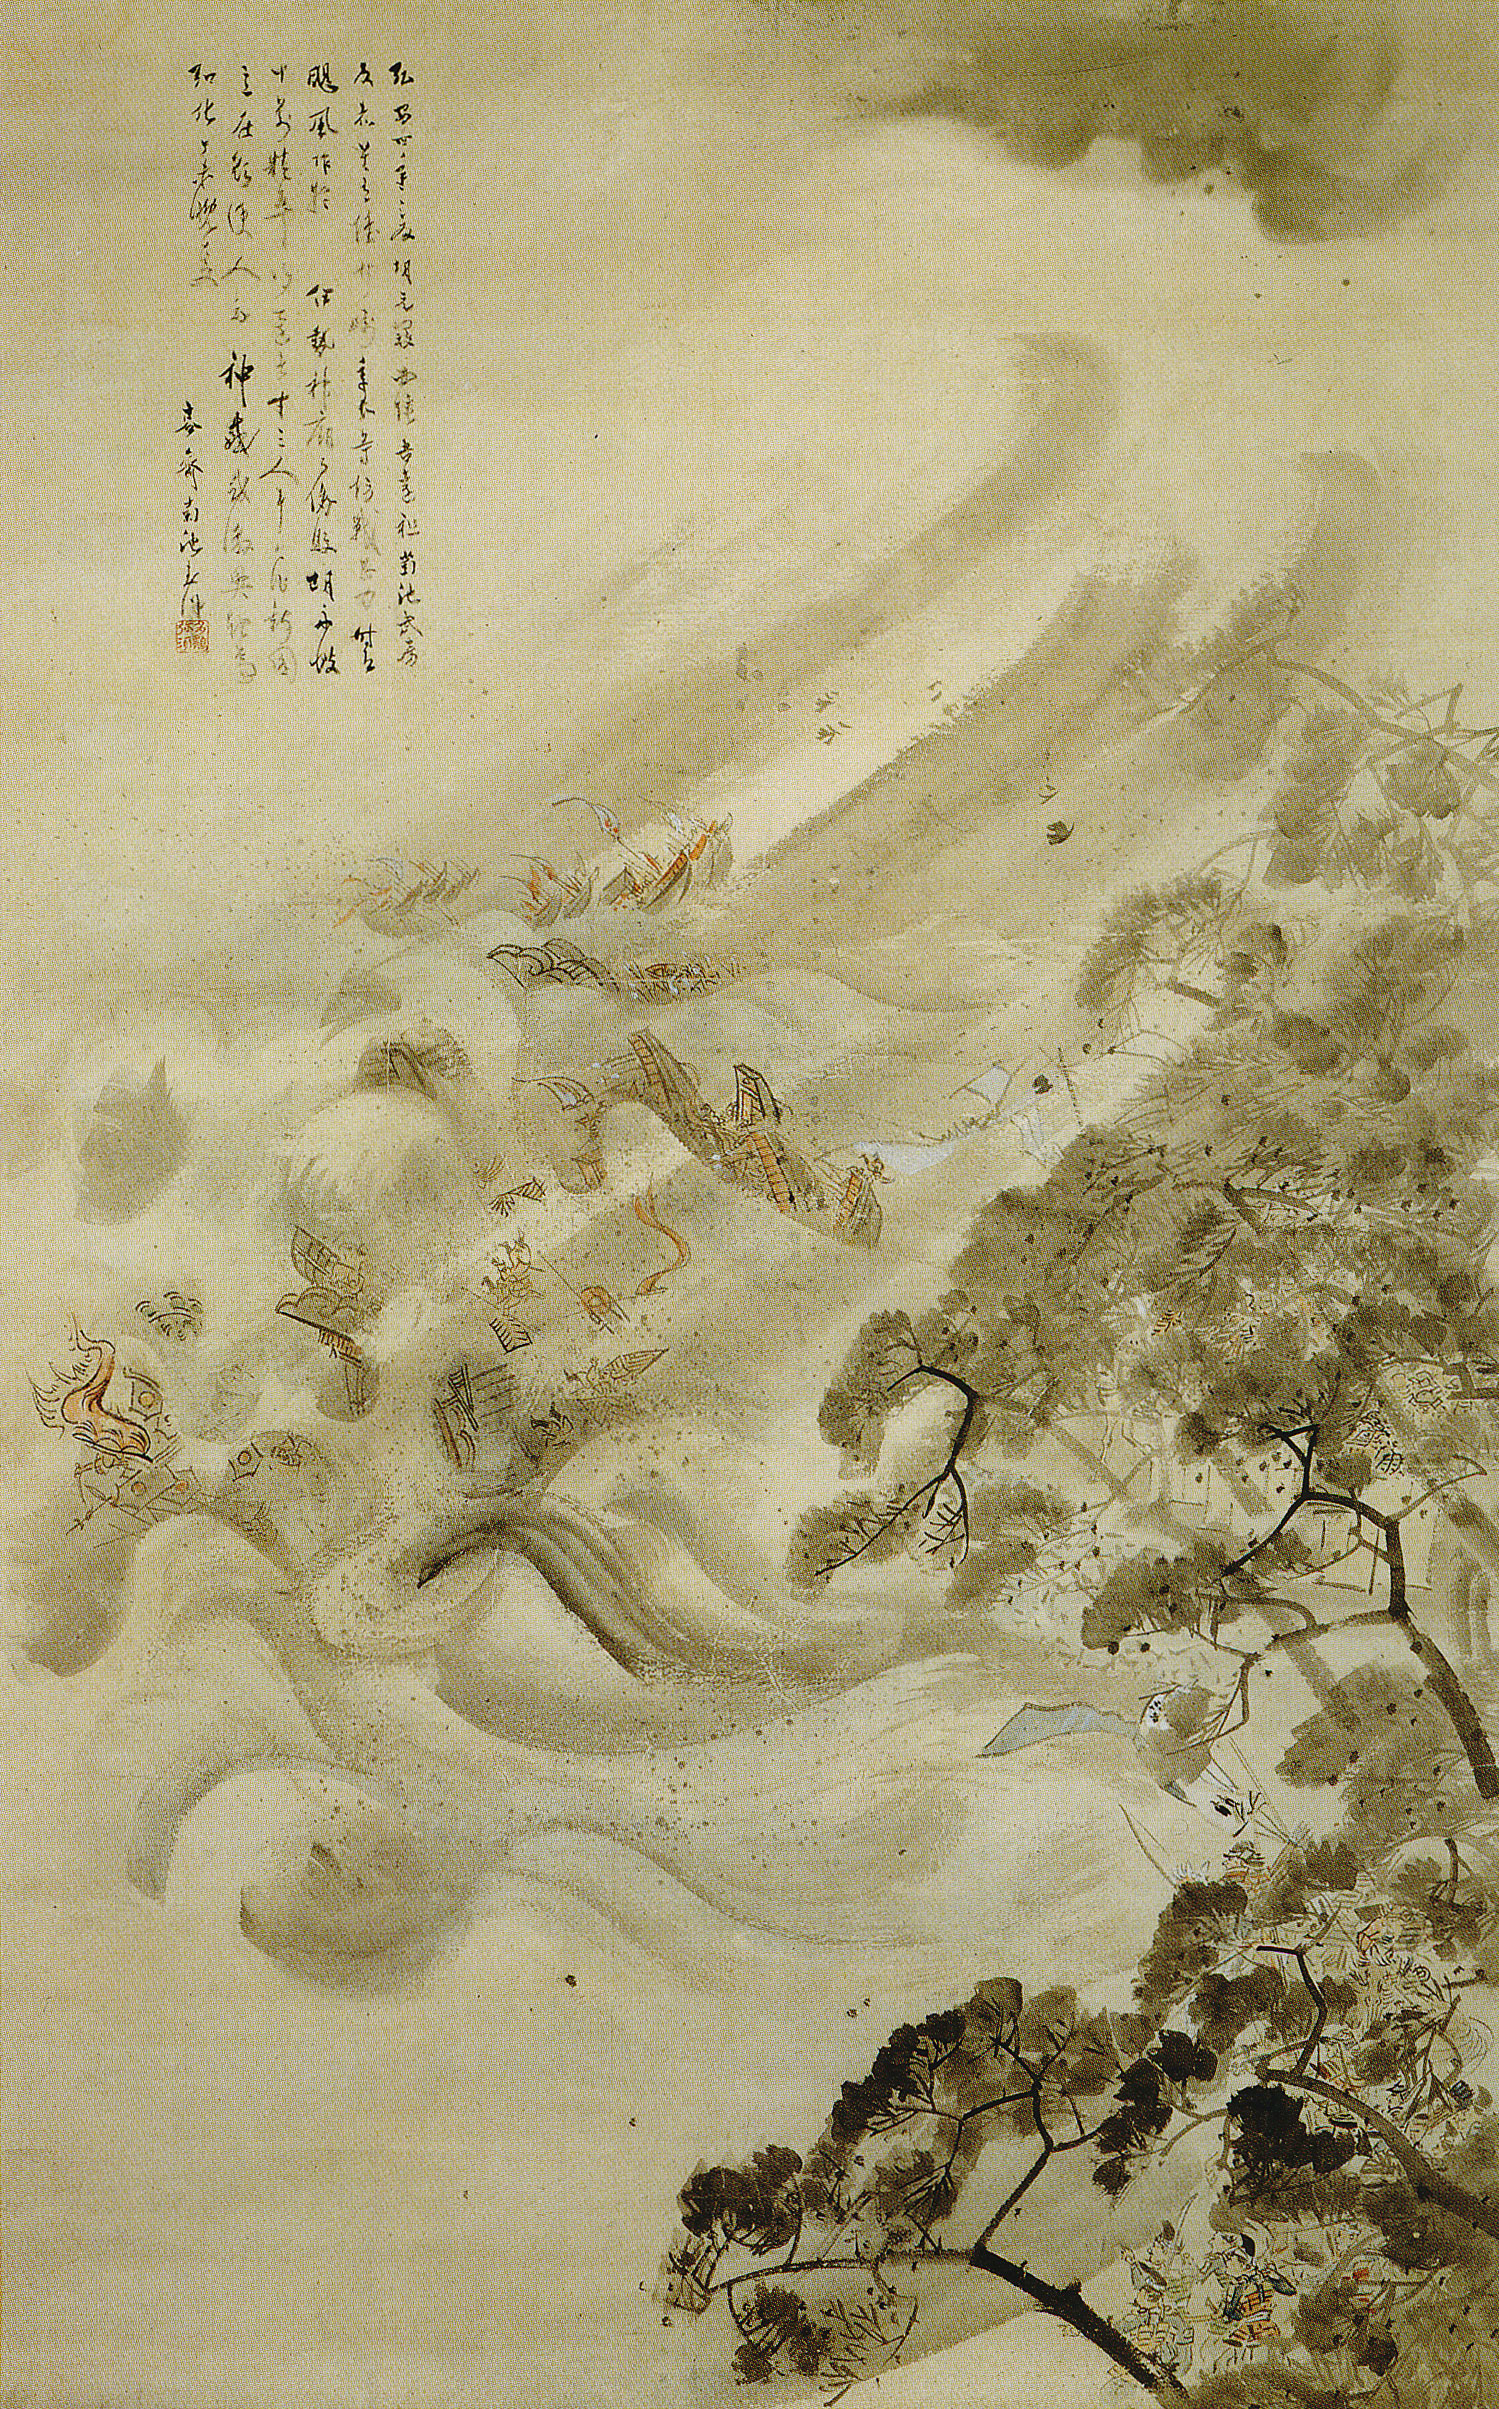
\includegraphics[width=0.38\textwidth]{MokoShurai.jpg}
    \caption{\small The Mongol fleet destroyed in a typhoon, ink and water on paper, by Kikuchi Y\={o}sai, 1847. 
    Source: Wikipedia}
    \label{fig:mongolJapan}
\end{wrapfigure}

\emph{Earth}, \emph{Wind}, \emph{Fire} \& \emph{Water}, the \emph{classical elements} were the basis 
for understanding our environment during antiquity. Modern science, based on experiments has taken a very 
different view of the world, one based on atoms, fundamental particles and states of matter. But we could 
argue that the classical elements were a more a philosophical idea that distilled our everyday experiences 
with nature, infact many ancient cultures such as Hellenistic Greece, Babylonia, Japan, Tibet, China and 
India had similar lists of four or five elements. These civilizations had very different views on the 
properties of these elements and how they related to natural phenomena, quite often these links 
were mythological. Indeed the obvious way in which people experienced the classical elements was through
weather systems. 

From the seasons to daily variations, nature's elements drive and shape our lives. Sometimes weather 
has had a direct impact on entire populations, one example was the failed Mongol invasions of Japan 
in $1274$ and $1281$. In both attacks, the Mongol fleets were almost entirely destroyed by storms called 
\emph{kamikaze} (translates to divine wind). Although some attacking Mongol forces did manage to land during 
the $1274$ campaign and outnumbered the defending armies, they were still defeated by Samurai clans with 
superior knowledge of the terrain. 

The invading fleet of $1281$ was composed of "more than four thousand ships bearing nearly $140,000$ men" 
\citep[pg.~17]{mcclain2002japan}, the scale of which was eclipsed only by the allied invasion of Normandy 
in 1944. The fleet was a hastily assembled, consisting of ships which were not suitable for the harsh waters 
between Japan and Korea. The Japanese had built two metre high walls in the intervening period and the invading 
fleets were forced to stay in sea for months. After their supplies were diminished, powerful kamikaze winds 
destroyed them entirely (an artists' view of the event is in figure \ref{fig:mongolJapan}). The failed invasions 
were a blow to the idea of Mongol supremacy in Asia and the Mongols never attemped an invasion of Japan since.

We now know that weather phenomena are caused by a combination of air pressure, temperature and moisture differences 
between one place and another. The angle of the Sun's rays changes with latitude, these variations create very 
different temperature trends from the poles to the equator. These differences in temperature lead to large scale 
air currents which create complex weather systems and climate patterns which we see across the world.

But weather phenomena are hardly exclusive to planet Earth.

\section*{The Final Frontier}

\begin{wrapfigure}{r}{0.4\textwidth}
    \centering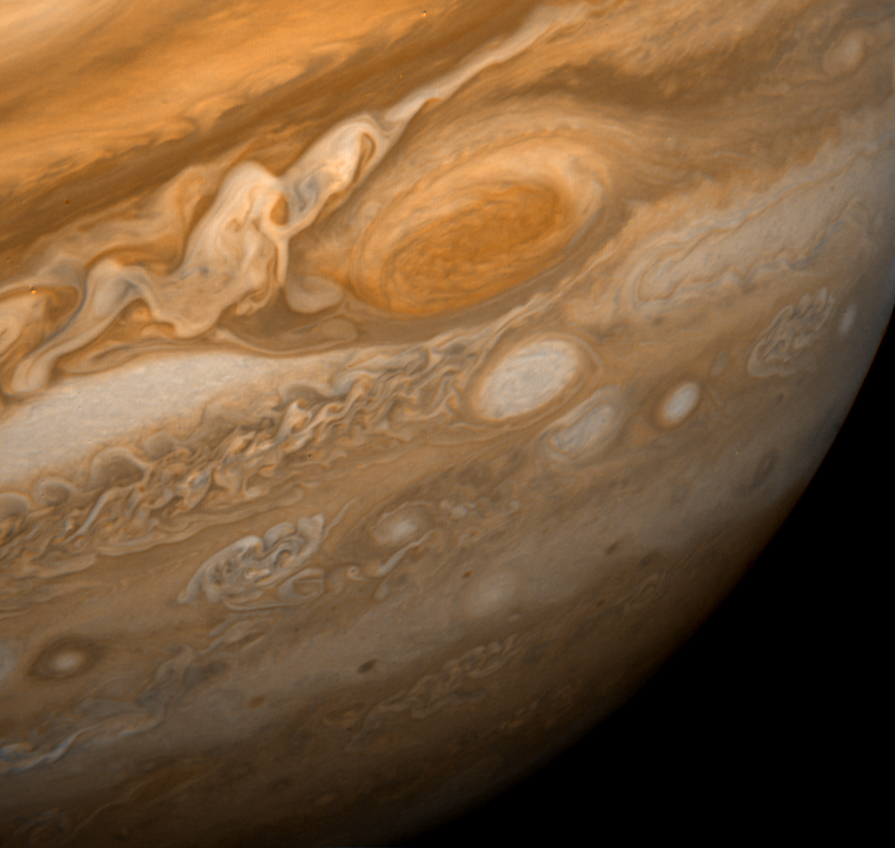
\includegraphics[width=0.38\textwidth]{Great_Red_Spot_From_Voyager_1.jpg}
    \caption{
        \small Jupiter's Great Red Spot in February 1979, photographed by the unmanned Voyager 1 NASA space probe. 
        Source: Wikipedia
    }
    \label{fig:jupiter}
\end{wrapfigure}

Even before the beginning of the space age, weather phenomena occurring on other planets have been observed. Jupiter's 
\emph{great red spot}, a huge storm, has been continuously observed since 1830 \citetext{see \citealp{britannicaRedSpot}}.
Saturn's \emph{great white spot}, a recurring storm system which was first used by Asaph Hall to determine the period of
the planet's rotation \citep{wikisaturn}. In the $20^{\text{th}}$ century, missions such as the Hubble space telescope, 
Voyager, Cassini and others have shown storms and other weather phenomena on planetary bodies like Venus, Mars, 
Neptune and Titan. 

The principles behind many planetary weather phenomena are very similar, their differences are because of the different 
compisition of each planet's atmosphere. Extra-terrestrial weather is just as complex and mind boggling as weather we 
observe on Earth, its scale is certainly much larger than we are used to. 

Yet, planetary weather is just one side of the puzzle. Venturing into our cosmic neighbourhood, our solar system
has another kind of weather system that has begun to be probed only very recently. 

\subsection*{A Gust of Wind from the Heavens}

During the last week of August 1859, several spots appeared on the surface of the Sun. Southern auroral displays were 
observed on August 29, as far north as Queensland Australia. Just before noon on September 1, British astronomer 
Richard Carrington observed a "white light flare" from a group of sun spots. He created a sketch of his observations
which is seen in figure \ref{fig:carringtonevent}. Carrington's observations were independently verified by British 
publisher and astronomer Richard Hodgson, both of them sent their reports to the 
\emph{Monthly Notices of the Royal Astronomical Society}.

September 1-2 1859 saw some remarkable events occur around the world. Auroral displays were observed all around the 
world, even in low latitude places such as Colombia \citep{MORENOCARDENAS2016257}. Auroras above the rocky mountains
in the U.S were so bright that they woke up gold miners who began preparing breakfast thinking it was morning 
\citep{miners}. In the northeastern U.S, people could read the newspaper by the aurora's light \citep{auroraReading}.

\begin{wrapfigure}{l}{0.4\textwidth}
    \centering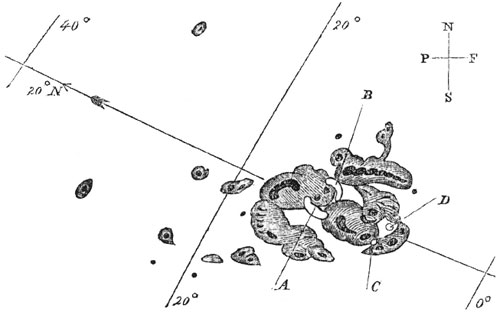
\includegraphics[width=0.38\textwidth]{Carrington_Richard_sunspots_1859.jpg}
    \caption{\small Sunspots of September 1, 1859, as sketched by Richard Carrington. 
    A and B mark the initial positions of an intensely bright event, 
    which moved over the course of five minutes to C and D before 
    disappearing. Source: Wikipedia}
    \label{fig:carringtonevent}
\end{wrapfigure}

The telegraph network in Europe and North America failed. Some operators experienced electric shocks 
\citep[pg.~13]{board2008committee} while in some cases even telegraph equipment that was disconnected 
from the power supply could be used to transmit messages \citep[pg.~58]{carlowicz2002storms}.

Based on global reports and observations taken by Scottish physicist Balfour Stewart at the 
Kew observatory in London, Carrington was able to connect events observed on the Earth to what 
he saw on the Sun on the $1^{\text{st}}$ of September \citep{clark2007sun}. His assertion was corraborated
by other observers in the scientific community.

The storm of 1859, later known as the \emph{Carrington event} was in some ways the genesis of \emph{Space Weather},
although the actual term was coined much later in the $1950$s. Although scientists had observed sunspots and their 
links to magnetic field variations on the Earth earlier, the \emph{Carrington event} was a concrete example of how 
activity on the Sun could have potentially dramatic effects on the Earth.

\subsection*{Space Weather}

\begin{wrapfigure}{r}{0.4\textwidth}
    \centering\includegraphics[width=0.38\textwidth]{induction_experiment.png}
    \caption{
        \small One of Faraday's 1831 experiments demonstrating induction. 
        The liquid battery (right) sends an electric current through the small coil (A). 
        When it is moved in or out of the large coil (B), its magnetic field induces a momentary 
        voltage in the coil, which is detected by the galvanometer (G). 
        Source: Wikipedia}
    \label{fig:induction}
\end{wrapfigure}

How do spots and ejections from the Sun produce bright lights and currents on Earth? During Carrington's time 
the fledgling science of Electromagnetism had picked up in the $19^{\text{th}}$ century and  already had some 
understanding of these phenomena. Faraday's induction experiment from 1831 (figure \ref{fig:induction}) had shown 
that varying magnetic fields could induce electrical currents in copper wires.

It took approximately a century from the \emph{Carrington event} for a theoretical understanding of Space 
Weather phenomena to develop. Maxwells equations of Electromagnetism \citep{maxwell1865viii} published in 
$1864$ gave scientists the mathematical tools to model the motions charged particles in electric and 
magnetic fields and the variations in the fields themselves due to those moving particles.

The $20^{\text{th}}$ century saw rapid progress made in modelling of charged particles in the Earth's magnetic 
field in the area of \emph{plasma physics}. Plasma was the name given to the state of matter containing 
positive and negatively charged particles in roughly equal numbers. Space weather started gaining relevance 
with the rise of space missions and satellites, though there was still much progress to be made. Physical 
theories about space plasmas needed to be combined with the data collected from space missions. This is 
especially important with the increasing reliance on electronic appliances and communication networks.

The Quebec power grid failure of 1989 \citep{kappenman1997geomagnetic} during a geomagnetic storm event showed 
that intense space weather events like the one observed in 1859 could cause significant damage to communications, 
energy and technological infrastructure that so crucial to the functioning of modern civilization.

But the solar storms observed in the $20^{\text{th}}$ and $19^{\text{th}}$ centuries are only one part of the 
picture. It is now increasingly likely that private companies will be making significant inroads into space 
travel for business goals. Companies such as SpaceX and BlueOrigin aim to make space travel cheaper and more 
accessible so that human beings can live and work in space or other planets in the solar system.

This drastic move to become a multi-planetary species will bring with it the risks to the human life and equipment. 
These risks come in the form of severe magnetic storms, solar flares and ejections of charged particles, which must 
be anticipated if we want to become a succesful space faring race. 

\subsection*{Space Science Informatics}



\clearpage
\bibliographystyle{plainnat}
\bibliography{references}
